\section{Linkages}
\begin{figure}[!htbp]
 \begin{center}
  \includegraphics{graphics/HumanTurkeyLinkage.pdf}
 \end{center}
\end{figure}

When graph drawings model physical objects, other qualities avout the graph can be contextualized in a geometric sense.  
Distance, angular relationstips and other geometric qualities of the drawings can be other useful properties of the drawing to perform analysis on.
The \textit{length assignment} of a graph $G=(V,E)$ is $\ell:E \mapsto \bbr^+$. 
For simple graphs, length assignment must be strictly positive, otherwise it may result in two distinct vertices with the same coordinates.
A \textit{linkage} is a graph $G = (V,E)$ with a length assignment $\ell:E \mapsto \bbr^+$.  
Length assignments can be thought of as a metric where $\ell(u,v) = \ell(v,u)>0$.
%Inser linkage here

Consider embeddings of a graph that respects the length assignment.  
A \textit{realization} of a linkage, $(G,\ell)$, is an embedding of a graph, $\Pi$, such that for every edge $\{u,v\} \in E$, $\ell\left( \{u,v\} \right) = \left\vert \Pi(u) - \Pi(v) \right\vert$.  
A \textit{plane realization} is a plane embedding with the property, $\ell\left( \{u,v\} \right) = \left\vert \Pi(u) - \Pi(v) \right\vert$.
First let's define the space of realizations for a corresponding linkage, i.e.:
$$P_{(G,\ell)} = \set{\Pi_{(G,\ell)}}{\forall \{u,v\} \in E\text{, }\ell\left( \{u,v\} \right) = \left\vert \Pi(u) - \Pi(v) \right\vert}$$
With respect to $P$, we can establish the a \textit{configuration space} that allows one to study problems of motion.  For each vertex of $G$, the embedding of the vertex lies in the plane, i.e. $\Pi(v) \in \bbR^2$.  By enumerating each vertex of $G$, e.g. $v_1, v_2, \dots, v_k, \dots, v_{n}$, we can create a projection mapping from $\mu: P \mapsto \bbR^{2\vert V \vert}$ where the corresponding coordinates of $\Pi(v_k)$ are in the $(2k)^\text{th}$ and $(2k+1)^{th}$ coordinates in $\bbR^{2\vert V \vert}$.  The configuration space is $\mu(P)$.  

By using real analysis, we can begin to pose problems about linkages with respect to a corresponding configuration space.  
We define a path $\gamma: [0,1]\mapsto \mu(P)$ where $\gamma(0)$ corresponds the the projection of a realization of a linkage $\Pi_0$ and $\gamma(1)$ corresponds to another realization of a linkage $\Pi_1$.  
If for any two elements $a,b \in \mu(P)$ that there exists a continuous path $\gamma$ such that $\gamma(0)=a$ and $\gamma(1)=b$, $\mu(P)$ is said to be path connected.   
For $\gamma$ to be continuous we would have that for every $\epsilon > 0$, there exists a $\delta >0$ such that if $x,y \in [0,1]$ and $\vert x-y \vert \delta$ then $\vlr{\vlr{\gamma(x)-\gamma(y)}}<\epsilon$.
$\gamma$ can be thought of as an animation of drawings that starts at $\gamma(0)$ and ends at $\gamma(1)$
To ask if $\mu(P)$ is a connected space, is to ask if $\mu(P)$ is connected in $\bbR^{2\vert V \vert}$.


%(fig 1) insert a table of a graph and define a length assigment 
%(fig 2) insert a realization of (fig 1)
%(fig 3) insert a second realization of (fig 1)



%graph component of the linkage   the plane.  A linkage 
%\textit{embedding} is $L : V \mapsto 
%\bbR^{2}$.
% A \textit{linkage} is an ordered pair $G = (V,E)$ comprising of a set $V$ of vertices or nodes 
% together with a set $E$ of edges or lines. This definition is commonly used for graphs.  Mapping 
% the linkage $G$ into the plane is said to be the \textit{embedding}, i.e. $L : V \mapsto 
% \bbR^{2}$.  A length function correspond to a linkage, $l: E \mapsto \bbr^+$ gives a length to an 
% edge in the linkage.  If We consider a \textit{realization} of a linkage is range of $L$, i.e. 
% $L(V)$. If for every edge $(u,v) \in E$ such that $l\left( \left(u,v\right) \right) = \left\vert 
% L(u) - L(v) \right\vert$ is true, then $L$ is said to be a \textit{proper embedding} of $G$.
% \begin{figure}[h]
% \begin{center}
% 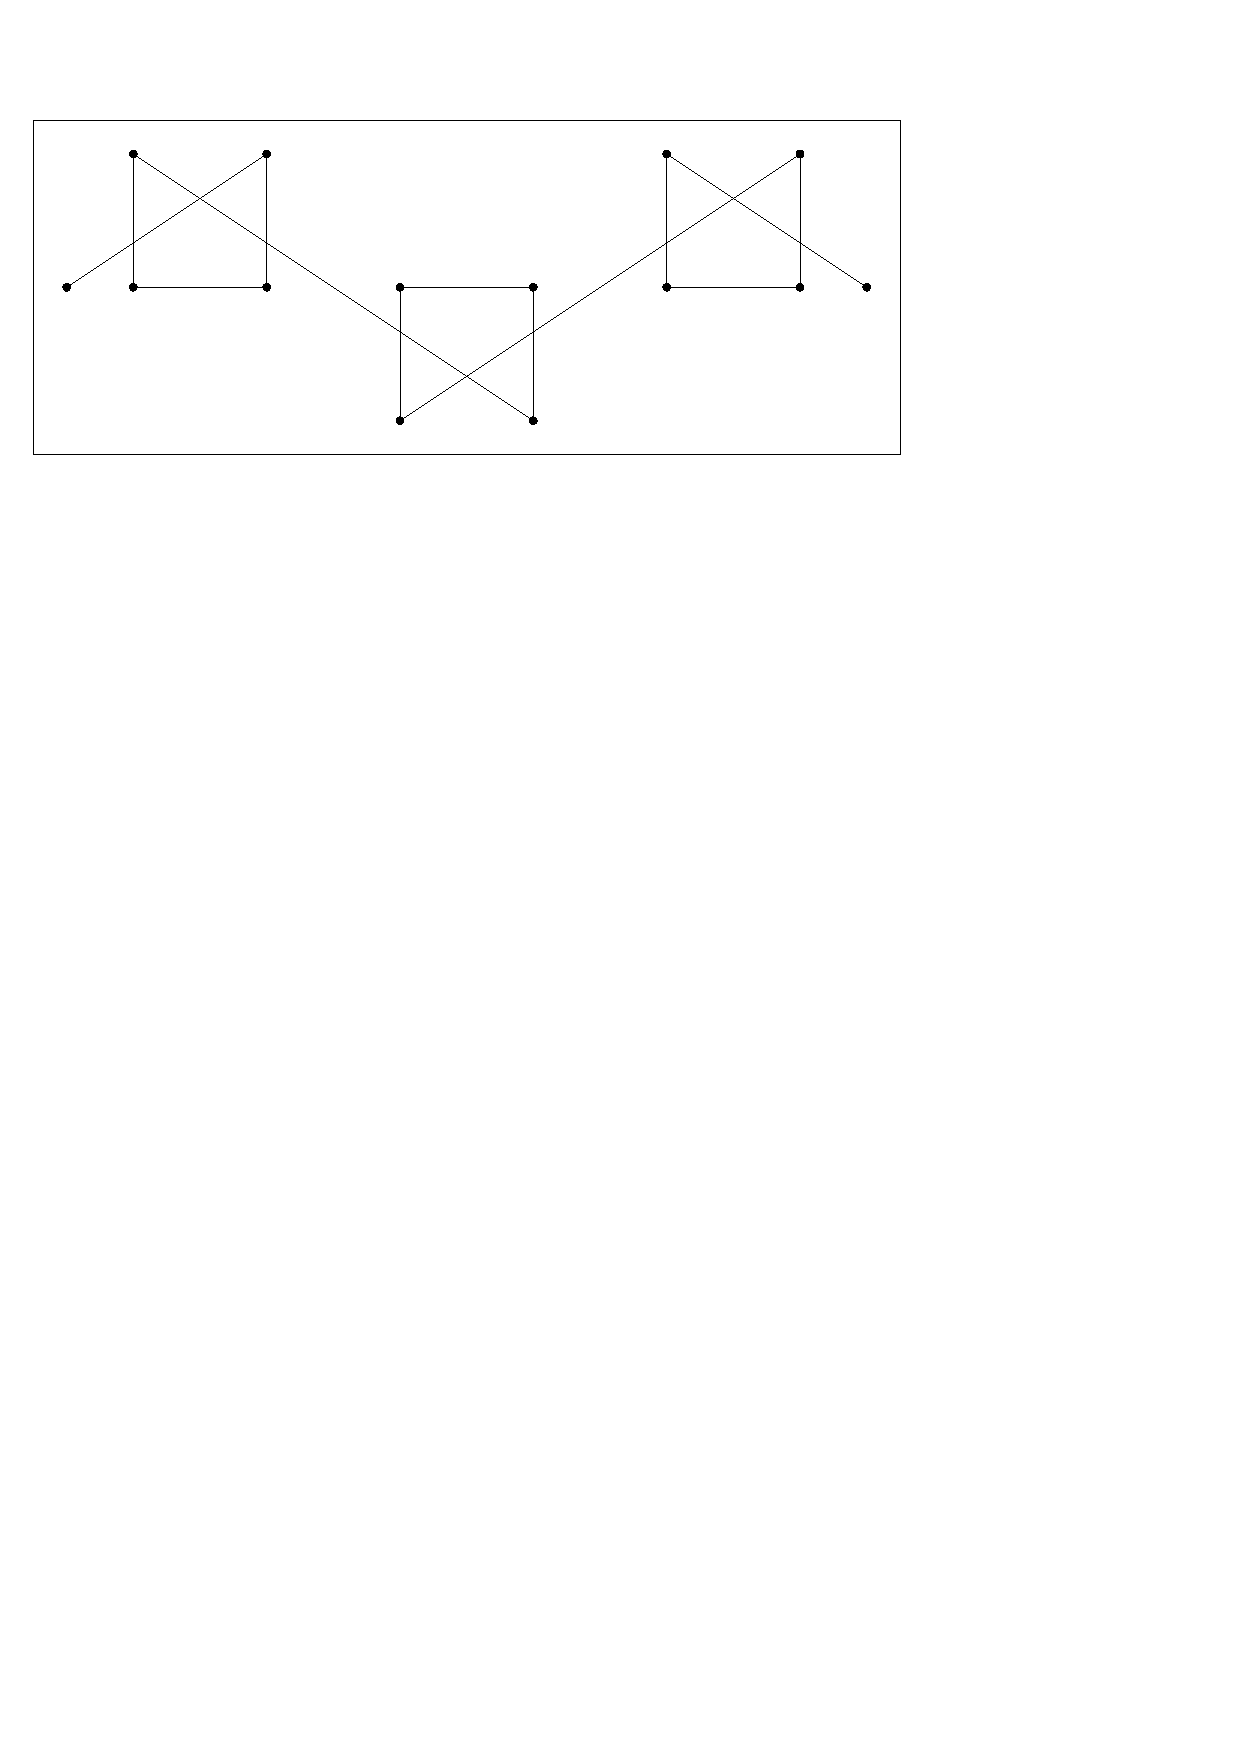
\includegraphics[scale=1]{graphics/crossingEdgeLinkage.pdf}
% \end{center} 
% \caption{A linkage where edges cross however it does not contain loops or multiple edges between 
% vertices.}
% \label{fig:linkage-3}
% \end{figure}
